\documentclass[12pt]{beamer}
\usepackage[utf8]{inputenc}
\usepackage[T1]{fontenc}
\usepackage{lmodern}
\usepackage{amsmath}
\usepackage{amssymb}

\usepackage{ulem}
\usepackage{booktabs}
\usepackage{xcolor}
\definecolor{myblue}{RGB}{94, 164, 233}     % Blue
\definecolor{myyellow}{RGB}{255, 204, 93}   % Yellow
\definecolor{mypink}{RGB}{249, 184, 184}    % Pink
\usepackage{graphicx}
\graphicspath{{./images/}}
\usetheme{default}
\usefonttheme{professionalfonts}
\usepackage[style=ieee, backend=biber]{biblatex}
\addbibresource{bibref.bib}

\setbeamertemplate{footline}{%
  \leavevmode%
  \hbox{\begin{beamercolorbox}[wd=.333333\paperwidth,ht=2.25ex,dp=1ex,center]{author in head/foot}%
    \usebeamerfont{author in head/foot}\insertshortauthor\hspace*{1em}
  \end{beamercolorbox}%
  \begin{beamercolorbox}[wd=.333333\paperwidth,ht=2.25ex,dp=1ex,center]{title in head/foot}%
    \usebeamerfont{title in head/foot}\insertshorttitle\hspace*{1em}
  \end{beamercolorbox}%
  \begin{beamercolorbox}[wd=.333333\paperwidth,ht=2.25ex,dp=1ex,right]{date in head/foot}%
    \usebeamerfont{date in head/foot}\insertshortdate{}\hspace*{2em}
    \insertframenumber{} / \inserttotalframenumber\hspace*{1ex}
  \end{beamercolorbox}}%
  \vskip0pt%
}

\begin{document}
	
	\author[Jesse Annan]{ {\small Presented by:} \newline {\Large Jesse Annan }}
	\title[SpanBERT]{SpanBERT: Improving Pre-training by Representing and Predicting Spans}
	\subtitle{
		{ \scriptsize \textbf{AUTHORS:} Mandar Joshi$^{*}$ \; Danqi Chen$^{*}$ \newline Yinhan Liu \; Daniel S. Weld \; Luke Zettlemoyer \; Omer Levy }
		}
	\institute{Department of Mathematics and Statistics \\  Georgia State University}
    \date{}
	
	\begin{frame}[plain]
		\maketitle
	\end{frame}
	
	\begin{frame}
		\frametitle{Outline}
		
		\tableofcontents
		
	\end{frame}
	
	\section{Background - The Rise of BERT}
	\begin{frame}
		\frametitle{Background}
		\framesubtitle{The Rise of BERT - Bidirectional Encoder Representations from Transformers}
		
		{ \large What is \textbf{BERT}? \cite{googlebert} } \newline
		
		\begin{itemize}
			\item \textbf{Bidirectional Context Understanding - }considers the context from the left and right sides of a word when predicting it representation %, allowing it to capture context for each word in a sentence.
			
			% BERT is built on the Transformer architecture, which was introduced in the paper "Attention is All You Need" 
			\item \textbf{Transformer Architecture - }uses self-attention mechanisms to weigh the importance of different words in a sentence when encoding their representations.	
		\end{itemize}
		
	\end{frame}
	
	\subsection{pre-training BERT}
	\begin{frame}
		\frametitle{Background}
		\framesubtitle{pre-training BERT}
		
		{ \large
			\textbf{BERT} optimizes two training objectives:
			
			\begin{itemize}
				\item Masked Language Model (MLM)
				\item Next Sentence Prediction (NSP)
			\end{itemize}
		}
	
		{ \large
			\vspace*{.5cm} 
			BERT is pre-trained on a large corpus of text data in an unsupervised manner. 
		}
		
	\end{frame}
	
	\subsection{Masked Language Model}
	\begin{frame}
		\frametitle{Background}
		\framesubtitle{Pre-training BERT - Masked Language Model}
		
		{ \large
			\textbf{MLM} is the task of predicting missing tokens in a sequence from their placeholders.
		} \newline
		
		\textbf{Implementation:} Given a sequence of word or sub-word tokens $\mathbb{X} = (x_1, x_2, \cdots, x_n)$
		\begin{enumerate}
			\setcounter{enumi}{-1}
			\item $\mathbb{Y}:= 15\% \; \mathbb{X}$
			\item replace 80\% (of $\mathbb{Y}$) with \textit{[MASK]}
			\item replace 10\% with a random token
			\item 10\% unchanged
		\end{enumerate}
		
	\end{frame}
	
	\subsection{Next Sentence Prediction}
	\begin{frame}
		\frametitle{Background}
		\framesubtitle{pre-training BERT - Next Sentence Prediction}
		
		{ \large
			\textbf{NSP} is the task of predicting weather a sequence is a direct continuation of another.
		} \newline
		
		\textbf{Implementation:} \cite{revspan} Sample two sequences $(\mathbb{X}_{A}, \mathbb{X}_{B})$. \newline $\mathbb{X}_{B}$ is:
		\begin{enumerate}
			\item 50\% of the time, the actual next sentence.
			\item 50\% of the time, a random sentence from the corpus
		\end{enumerate}
		
	\end{frame}
	
	\begin{frame}
	\frametitle{Background}
	\framesubtitle{BERT - Summary and Limitation}
		
		{ \large
			\textbf{BERT} optimizes the \textbf{MLM} and \textbf{NSP} objectives by masking word pieces uniformly at random in data generated by the bi-sequence sampling procedure.	\newline \newline
		}	
			\textit{*Falls short in understanding spans of text.}
		
	\end{frame}
	
	\section{SpanBERT}
	\begin{frame}
		\frametitle{SpanBERT}
		\framesubtitle{Improving Pre-training by Representing and Predicting Spans}
		
		{ \large
			\textbf{SpanBERT} \cite{metasbert} is a pre-training method that is designed to better represent and predict spans of text.
		} \newline
		
		\begin{itemize}
			\item mask spans of token, rather than individual ones
			\item *predict spans using representations from span boundaries
			\item \sout{NSP}, samples a single segment of text for each training example
		\end{itemize}
		
	\end{frame}
	
	\subsection{Span Masking}
	\begin{frame}
		\frametitle{SpanBERT}
		\framesubtitle{Span Masking Objective (similar to MLM)}
		
		Sample a number of (complete) words from a geometric distribution, $l \sim Geo(p = 0.2)$, clipped at $l_{max} = 10$
		
		\begin{figure}
			\centering
			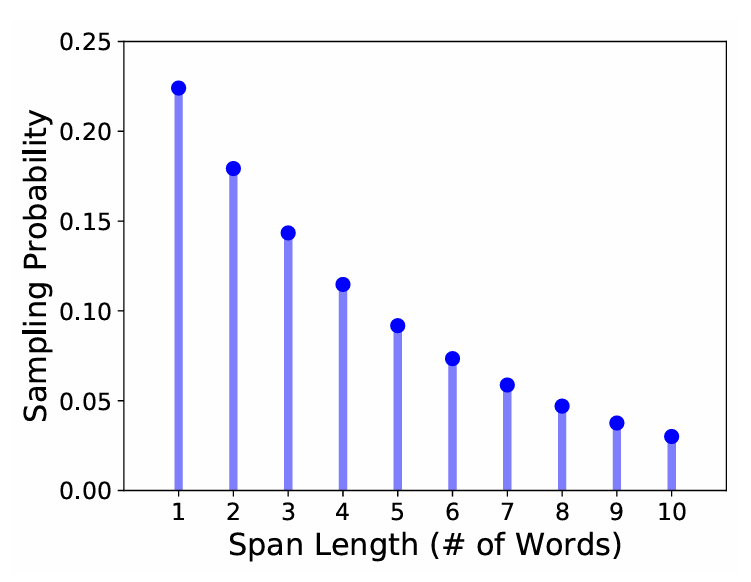
\includegraphics[width=.7\textwidth]{spanlength.png}
		\end{figure}
		
		{ \small
			\textit{mean($l = 3.8$); experimented with p =\{0.1, 0.2, 0.4\}}
		}
		
	\end{frame}
	
	\subsection{Span Boundary Objective}
	\begin{frame}
		\frametitle{SpanBERT}
		\framesubtitle{Span Boundary Objective (SBO)}
		
		{ \large
			\textbf{SBO} involves predicting each token of a masked span using only the representations of the observed tokens at the boundaries.
		} \newline
		
		Given a masked span of tokens $(x_{s}, . . . , x_{e}) \in \mathbb{Y}$ \newline
		\[ \mathbf{y}_{i} = f ( \mathbf{\textbf{x}}_{s-1}, \; \mathbf{\textbf{x}}_{e+1}, \; \mathbf{\textbf{p}}_{i-s+1} ) \]
		
		where $x_i$ is the ith token in the masked span, $\mathbf{\textbf{x}}_i$ is the output of the transformer encoder for ith token in the sequence, and $f$ is a 2-layer feed-forward network with GeLU actiation function \cite{gelu} and Layer Normalization \cite{normlayer}.
		
	\end{frame}
	
	\begin{frame}
		\frametitle{SpanBERT}
		\framesubtitle{Span Boundary Objective (SBO) Cont'd}
			
		\begin{equation*}
			\begin{split}
				\textbf{h}_{0} & = [ \mathbf{\textbf{x}}_{s-1}, \; \mathbf{\textbf{x}}_{e+1}, \; \mathbf{\textbf{p}}_{i-s+1} ] \\
				\textbf{h}_{1} & = \text{LayerNorm}( \text{GeLU}( \textbf{W}_{1} \textbf{h}_{0} )) \\
				\mathbf{y}_{i} & = \text{LayerNorm}( \text{GeLU}( \textbf{W}_{2} \textbf{h}_{1} ))
			\end{split}
		\end{equation*}
		
		 $\mathbf{y}_{i}$ to predict the token $x_{i}$ and compute the cross-entropy loss.
		 \begin{equation*}
		 	\begin{split}
		 		\mathcal{L} & = \mathcal{L}_{MLM}(x_i) + \mathcal{L}_{SBO}(x_i) \\
		 		& = - log P(x_i | \mathbf{\textbf{x}}_i) - log P(x_i | \mathbf{y}_i)
		 	\end{split}
		 \end{equation*}
		
	\end{frame}

        \begin{frame}
            \frametitle{GeLU Activation Function}
            \framesubtitle{GeLU v.s. ReLU v.s. ELU}

            \begin{figure}
			\centering
			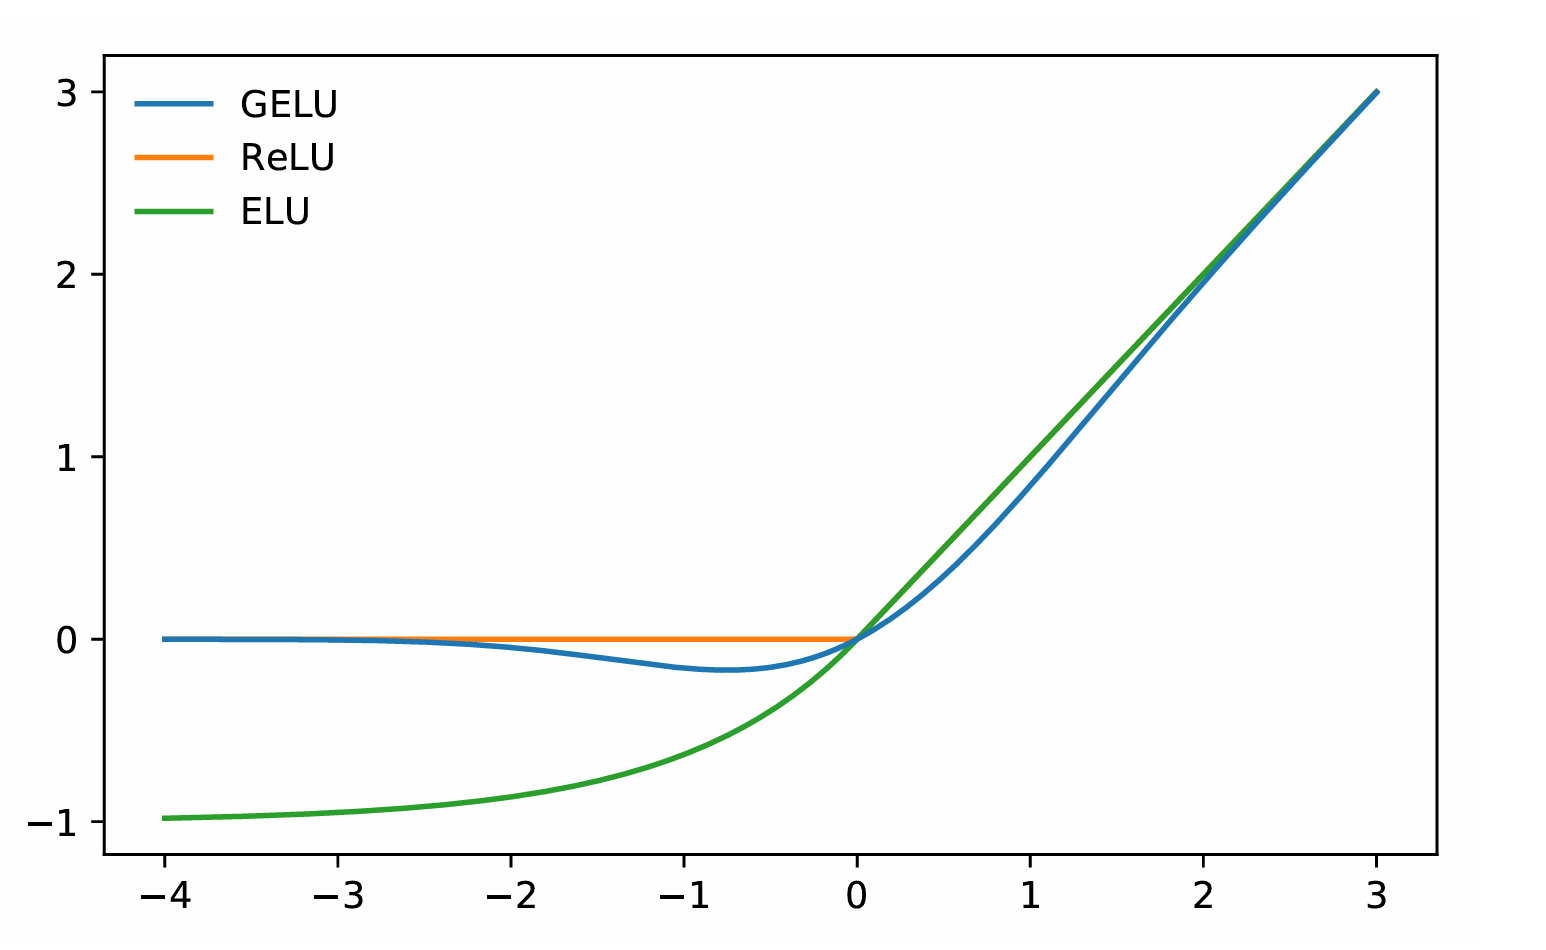
\includegraphics[width=.65\textwidth]{gelu.png}
                \caption{The GELU ($\mu = 0, \sigma = 1$), ReLU, and ELU ($\alpha$ = 1)}
		\end{figure}

            GeLU has shown good empirical performance in various deep learning tasks, including NLP. It is a popular choice in transformer-based models.
            
        \end{frame}
 
	\subsection{Single-sequence v.s. Bi-sequence}
	\begin{frame}
		\frametitle{SpanBERT}
		\framesubtitle{Single-sequence v.s. Bi-sequence training}
		
		\begin{itemize}
			\item \textbf{SpanBERT} samples a single contiguous segment of up to $n = 512$ instead of using NSP which uses two segments for pretraining, as in \textbf{BERT}. \newline
			
			\item It is conjectured that \textbf{single-sequence training is superior to bi-sequence training} with NSP because
			\begin{enumerate}
				\item the model benefits from longer full-length contexts, or 
				\item conditioning on, often unrelated, context from another document adds noise to the MLM.
			\end{enumerate}
		\end{itemize}
		
	\end{frame}
	
	\subsection{SpanBERT Framework}
	\begin{frame}
		\frametitle{SpanBERT}
		\framesubtitle{SpanBERT Framework}
		
		\begin{figure}
			\centering
			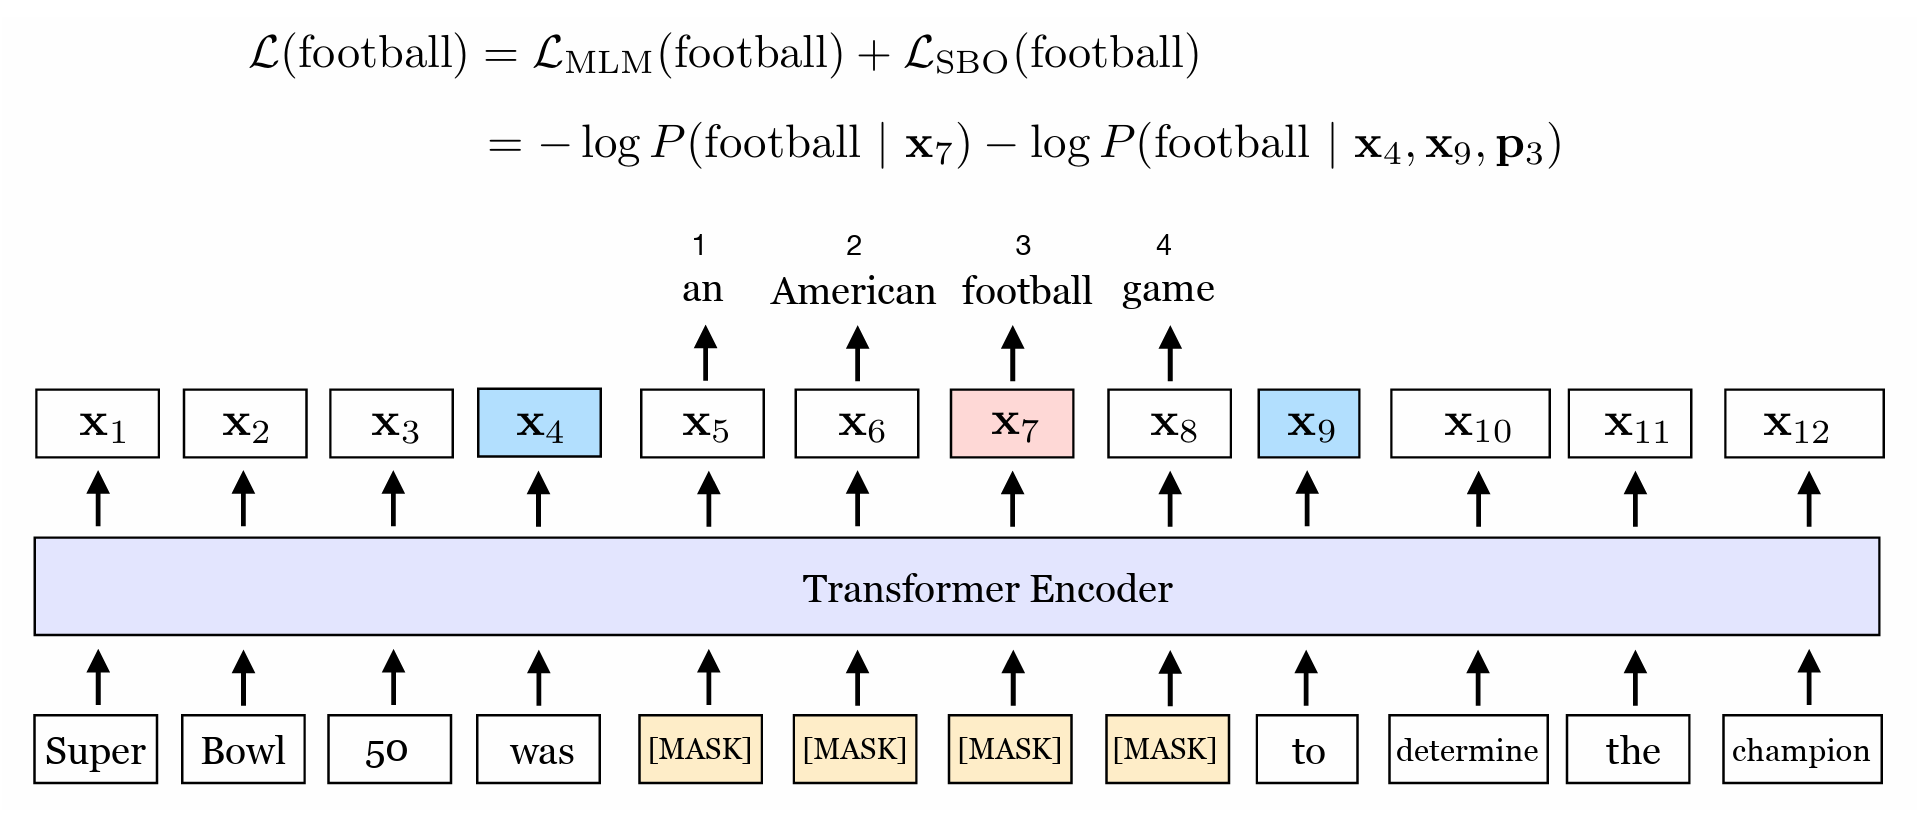
\includegraphics[width=.93\textwidth]{spanbert.png}
			\caption{ The span \textcolor{myyellow}{an American football game} is masked. The SBO uses \textcolor{myblue}{$\mathbf{\textbf{x}}_{4}$} and \textcolor{myblue}{$\mathbf{\textbf{x}}_{9}$}, to predict each token in the masked span. The equation shows the loss terms for predicting the token, \textcolor{mypink}{football}, marked by the position embedding $\mathbf{\textbf{p}}_{3}$.}
		\end{figure}
		
	\end{frame}
	
	\section{Experiments}
	\subsection{Span Related Tasks}
	\begin{frame}
		\frametitle{SpanBERT: Experiments}
		\framesubtitle{Span Related Tasks}
		
		\large
		\begin{itemize}
			\item Extractive Question Answering \newline
			\item Coreference Resolution \newline
			\item Relation Extraction \newline
		\end{itemize}
	
	\end{frame}	
	
	\subsection{Experiment Baselines}
	\begin{frame}
		\frametitle{SpanBERT: Experiments}
		\framesubtitle{Baselines}
		
		\large
		\begin{itemize}
			\item \textbf{Google BERT} - original BERT (results) \newline
			\item \textbf{Our BERT} - reimplementation of BERT; used different mask at each epoch \newline
			\item \textbf{Our BERT-1seq} - reimplementation of BERT; used single full-length sequences (\sout{NSP})
 		\end{itemize}
		
	\end{frame}	
	
	\subsection{Results}
	\begin{frame}
		\frametitle{SpanBERT: Experiments}
		\framesubtitle{Extractive Question Answering - SQuAD 1.1/2.0 benchmark}
		
		\begin{figure}
			\centering
			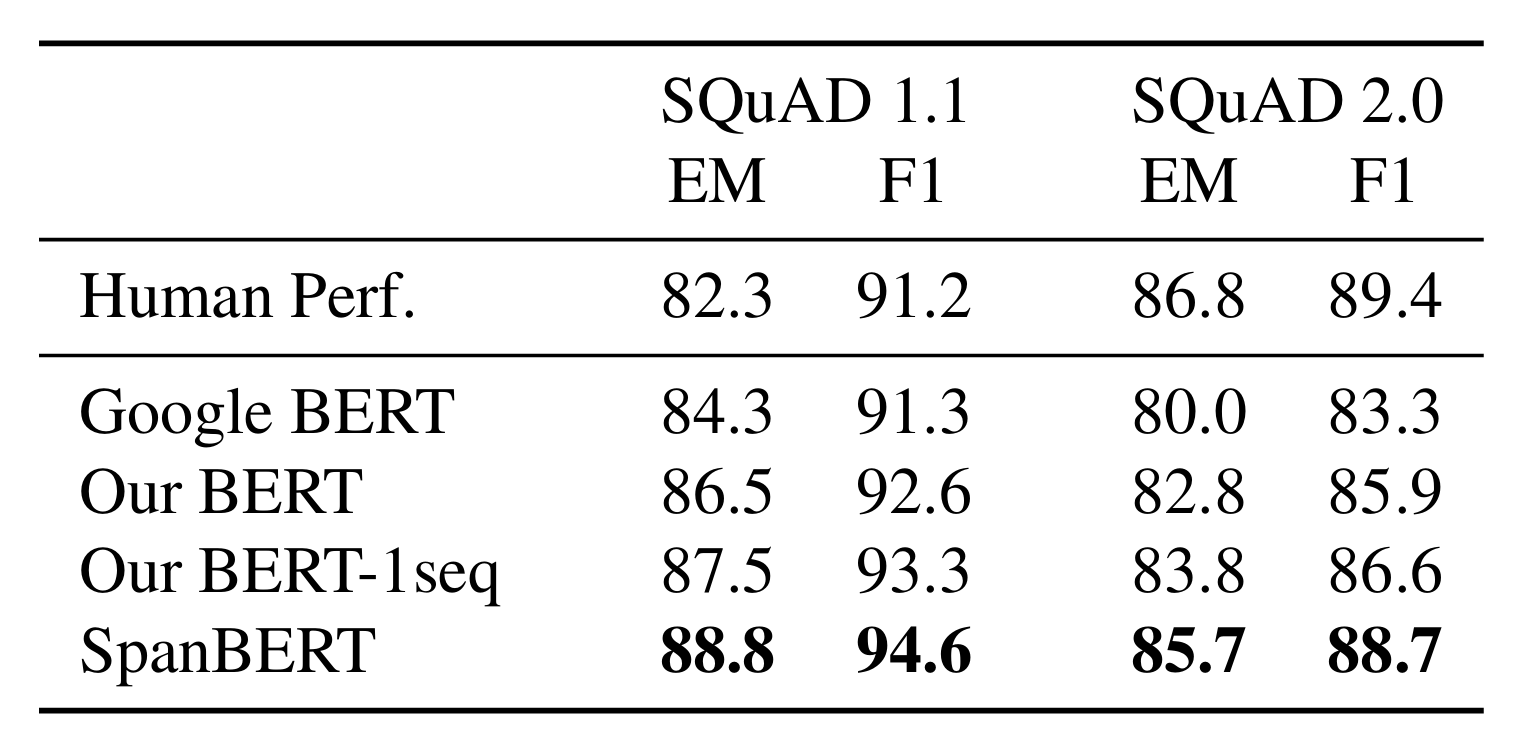
\includegraphics[width=\textwidth]{qa1.png}
			\caption{\textbf{SpanBERT} exceeds the \textbf{our BERT} baseline by 2.0\% and 2.8\% F1, respectively. Also 3.3\% and 5.4\% over \textbf{Google BERT}}
		\end{figure}
		
	\end{frame}	
	
	\begin{frame}
		\frametitle{SpanBERT: Experiments}
		\framesubtitle{Extractive Question Answering - MRQA benchmark}
		
		\begin{figure}
			\centering
			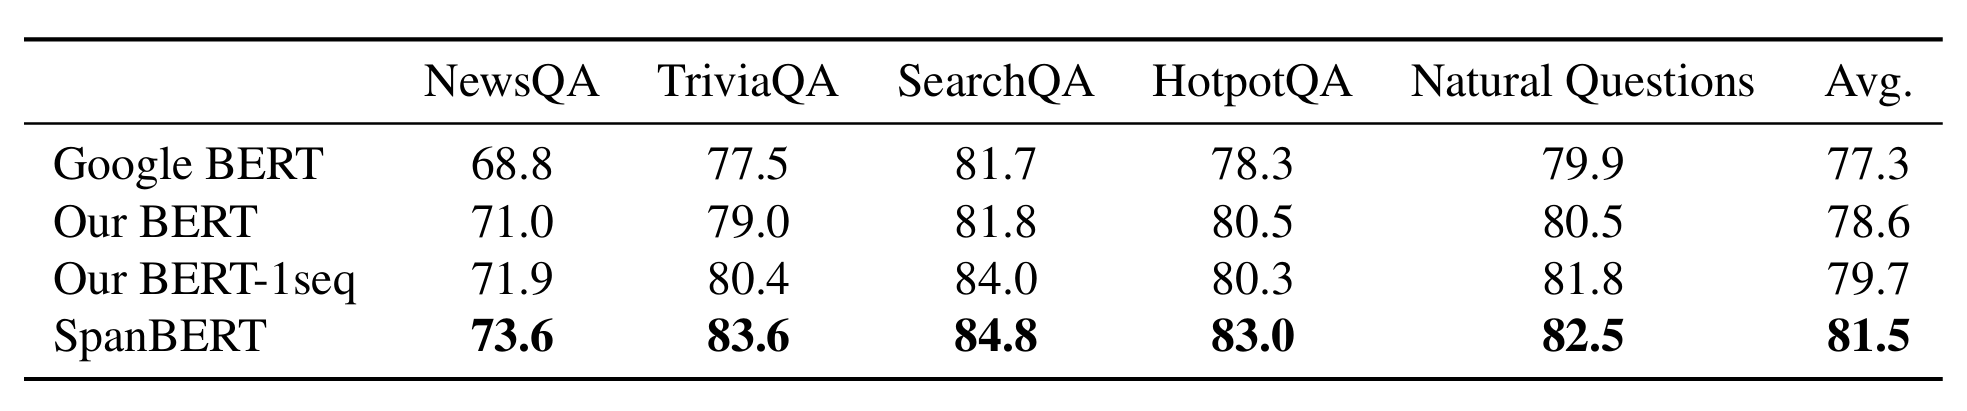
\includegraphics[width=\textwidth]{qa2.png}
			\caption{Performance (F1) on the five MRQA extractive question answering tasks. On average, we see a 2.9\% F1 improvement from reimplementation of \textbf{BERT}}
		\end{figure}
		
	\end{frame}	
	
	\begin{frame}
		\frametitle{SpanBERT: Experiments}
		\framesubtitle{Coreference Resolution - OntoNotes benchmark}
		
		\begin{figure}
			\centering
			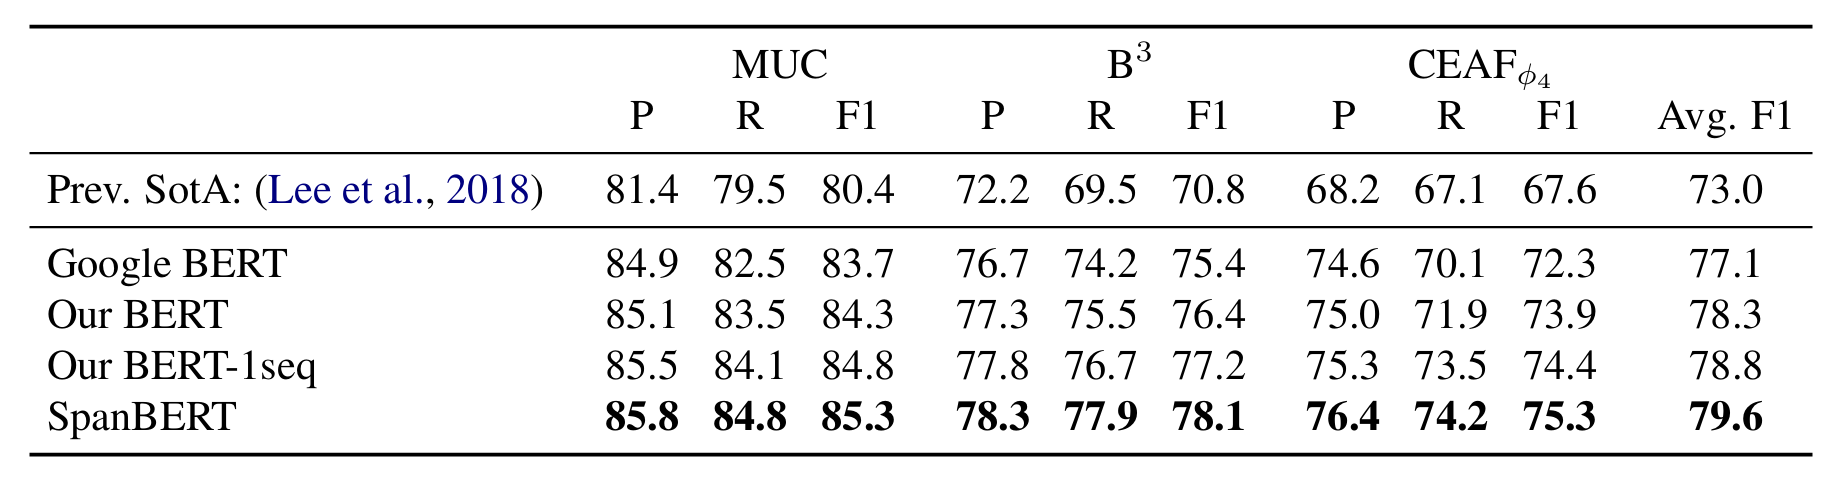
\includegraphics[width=\textwidth]{cres.png}
			\caption{\textbf{SpanBERT} achieves a new state of the art (SotA) of 79.6\% F1}
		\end{figure}
		
	\end{frame}	
	
	\begin{frame}
		\frametitle{SpanBERT: Experiments}
		\framesubtitle{Relation Extraction - TACRED benchmark}
		
		\begin{figure}
			\centering
			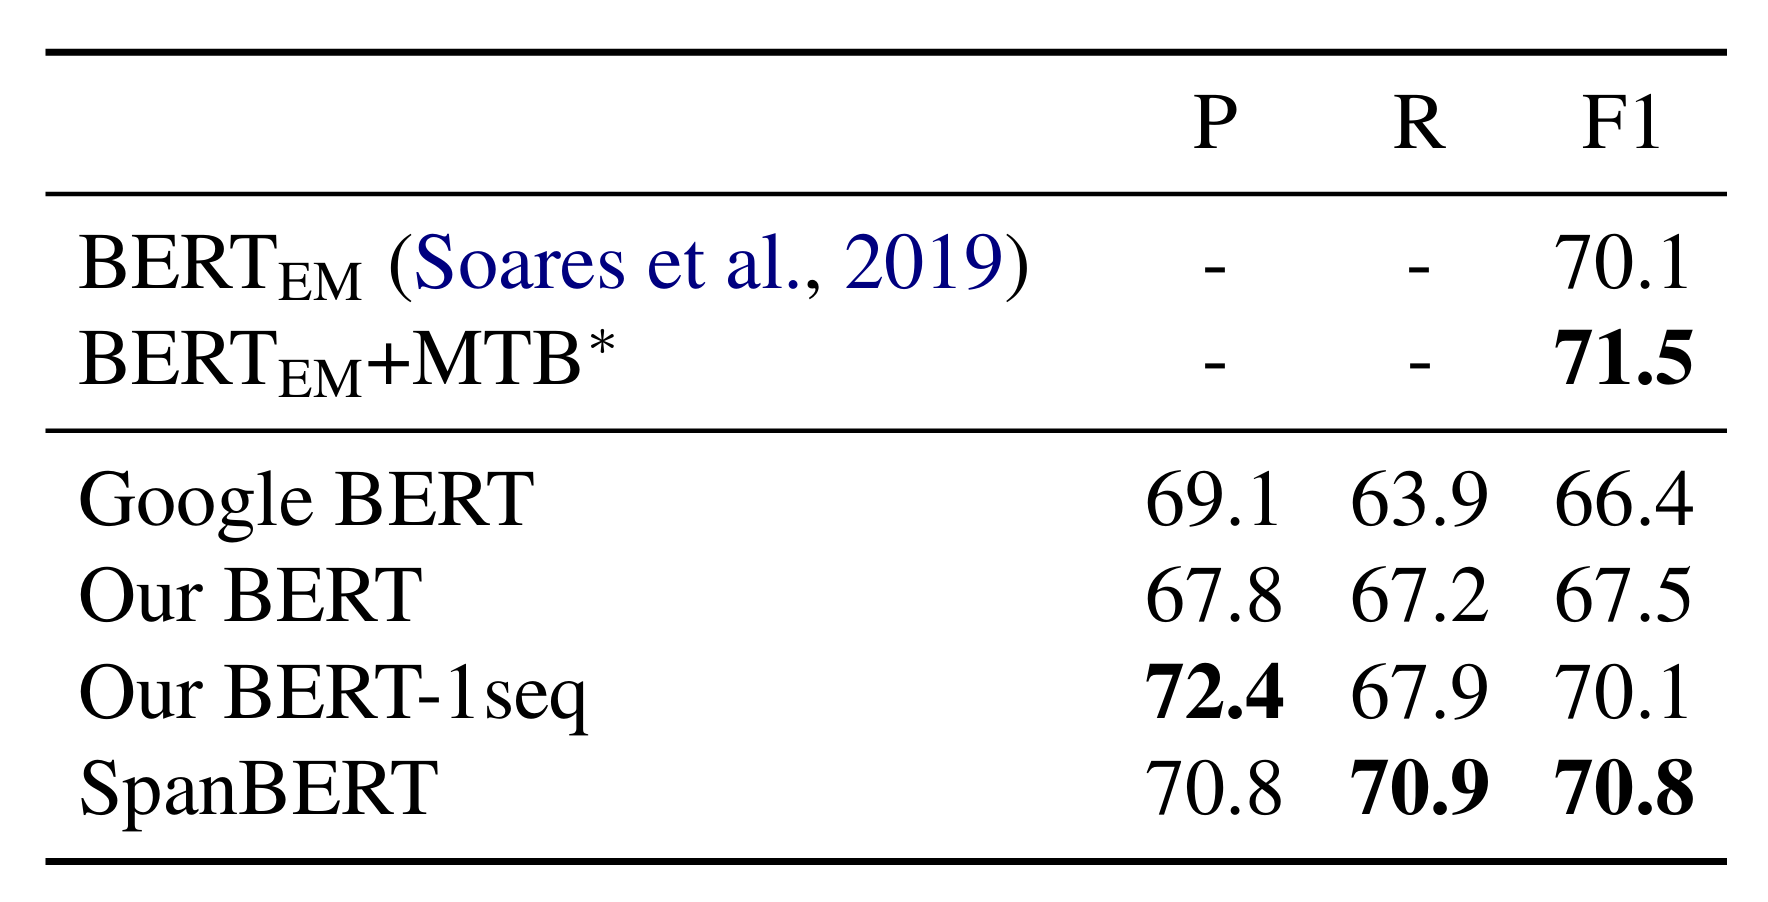
\includegraphics[width=\textwidth]{rele.png}
			\caption{\textbf{SpanBERT} exceeds the reimplementation of \textbf{BERT} by 3.3\% F1 and achieves close to the current SotA}
		\end{figure}
		
	\end{frame}	

    \begin{frame}
        \frametitle{GLUE}
        \framesubtitle{The General Language Understanding Evaluation (GLUE) benchmark}

        \begin{figure}
			\centering
			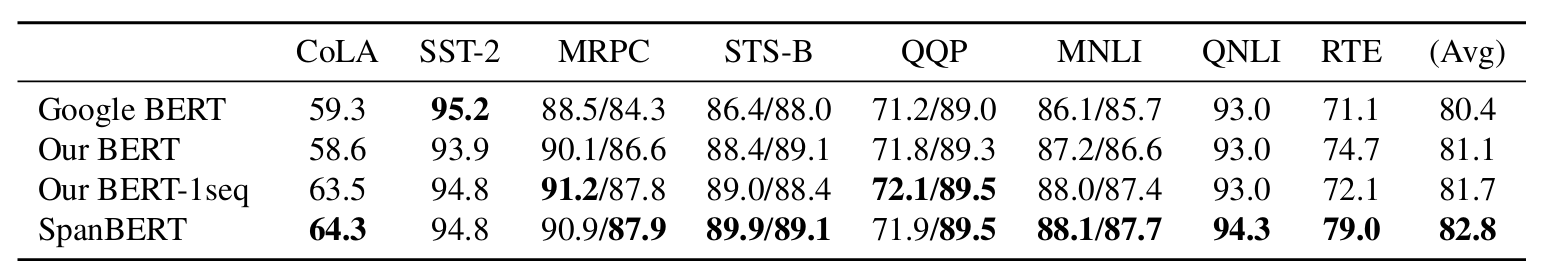
\includegraphics[width=\textwidth]{glue.png}
			\caption{Test set performance on GLUE tasks. MRPC: F1/accuracy, STS-B: Pearson/Spearman correlation, QQP: F1/accuracy, MNLI: matched/mismatched accuracies and accuracy for all the other tasks}
		\end{figure}
        
    \end{frame}
 
	\begin{frame}
		\frametitle{SpanBERT: Experiments}
		\framesubtitle{Ablation Studies on masking schemes}
		
		\begin{figure}
			\centering
			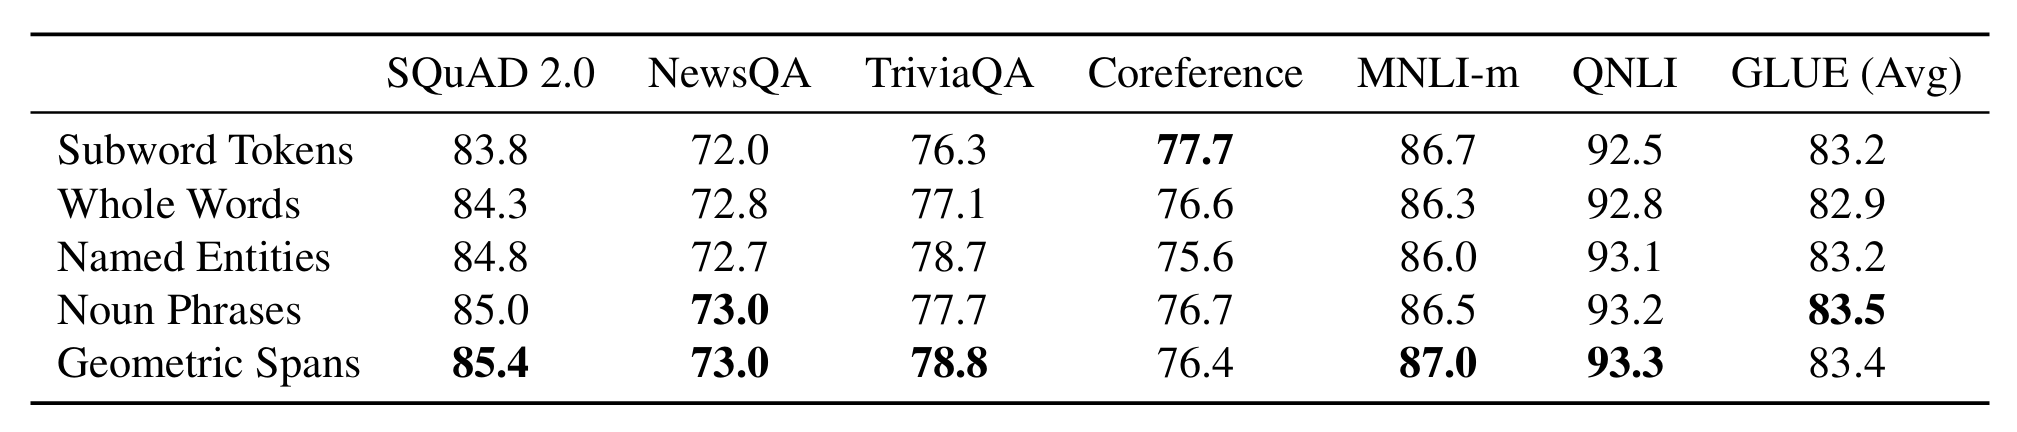
\includegraphics[width=\textwidth]{abla1.png}
			\caption{The effect of replacing \textbf{BERT}'s original masking scheme (subword tokens). \textbf{SpanBERT} geometric spans outperforms other span variants (F1 scores). All the models are based on bi-sequence training with NSP}
		\end{figure}
		
	\end{frame}	
	
	\begin{frame}
		\frametitle{SpanBERT: Experiments}
		\framesubtitle{Ablation Studies on auxiliary objectives}
		
		\begin{figure}
			\centering
			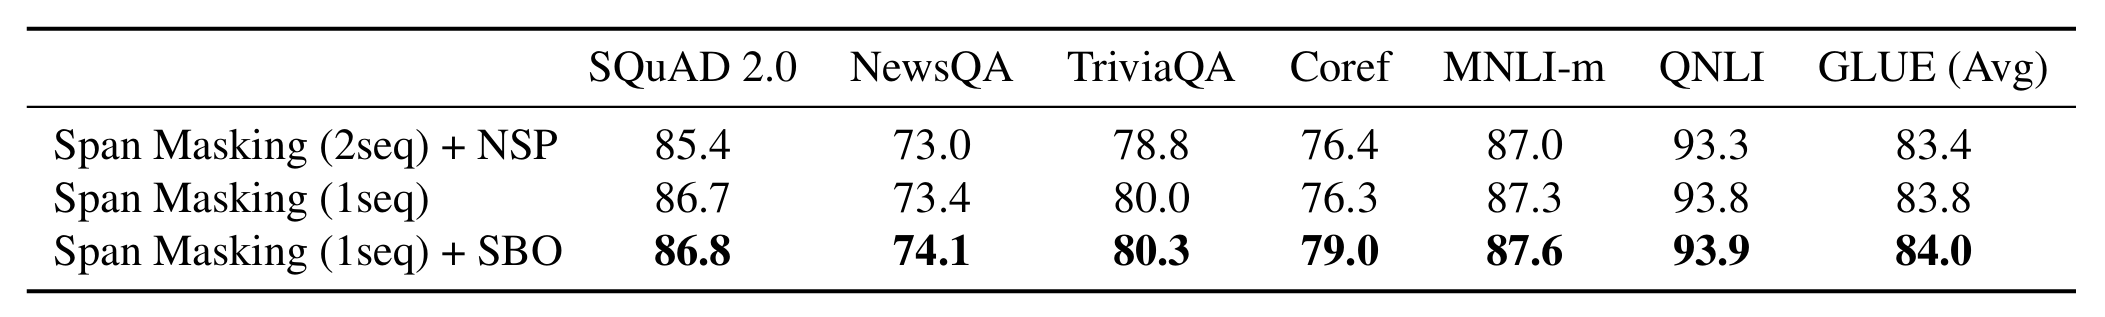
\includegraphics[width=\textwidth]{abla2.png}
			\caption{The effect of different auxiliary objectives. Single-sequence training typically improves performance, adding SBO further improves performance.}
		\end{figure}
		
	\end{frame}	
	
	\section{Conclusion}
	\begin{frame}
		\frametitle{SpanBERT}
		\framesubtitle{Conclusion and Observations}
		\large
		In Summary, \textbf{SpanBERT}: \newline
		\begin{enumerate}
			\item masking spans of full words using a geometric distribution based masking scheme.
			\item optimizing an auxiliary span-boundary objective in addition to MLM using a single-sequence data pipeline. 
			\item better at extractive question answering. 
			\item single-sequence training works considerably better than bi-sequence training with NSP.
		\end{enumerate}
		
	\end{frame}

    \section{References}
    \begin{frame}[allowframebreaks]{Resources}
        
        \printbibliography
        
    \end{frame}

    \begin{frame}
        
        \vfill
        \begin{center}
             \Huge \textbf{Q \& A}
             \rule{\linewidth}{1.5pt} \newline
             \Huge \textbf{Thank You!}
        \end{center}
        \vfill
        
    \end{frame}
 
\end{document}